\section{Introduction}
\label{sec:intro}

\begin{figure}[t]
  \centering
  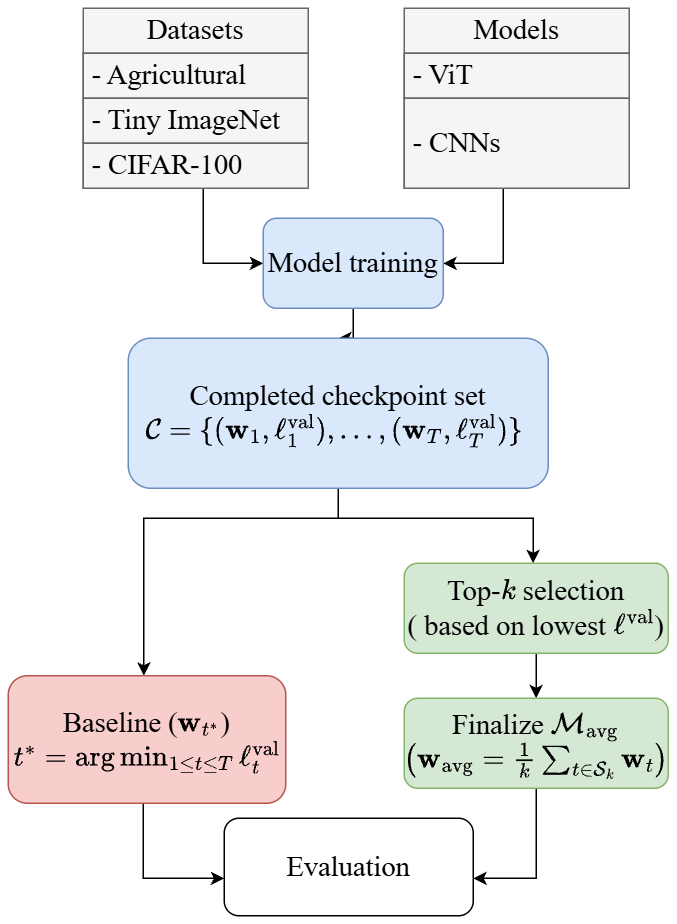
\includegraphics[width=\linewidth]{Pipeline.png}
  \caption{The rule operates only at the model-selection stage. Training runs
    unmodified and emits a checkpoint set; the baseline keeps the single
    best-scoring state, while we keep the top $k$ by the same criterion, average
    their trainable parameters, and recompute Batch-Normalization statistics
  before the final evaluation.}
  \label{fig:pipeline}
\end{figure}

Nearly every supervised vision pipeline ends with the same step. Training
produces a sequence of epoch checkpoints, each is scored on a held-out
validation split, and the single best-scoring state is kept as the final model
\cite{bishop2006pattern,prechelt2002early}. The step is so routine that it is
rarely reported, let alone questioned. Yet it is a winner-takes-all decision
taken on a noisy statistic: late-epoch validation metrics fluctuate under
mini-batch sampling, stochastic optimization, and the finite size of the
validation split \cite{prechelt2002early,izmailov2019averagingweightsleadswider,garipov2018losssurfacesmodeconnectivity},
and checkpoints with near-identical training loss can generalize
measurably differently \cite{keskar2017largebatchtrainingdeeplearning}. The gap
between the best and second-best epoch is often well inside that noise, so
which one wins is partly an accident of the run.

Aggregating several states rather than committing to one is the natural
response. Prediction-time ensembling does this but multiplies inference cost by
the ensemble size \cite{dietterich2000ensemble}. Weight averaging avoids that:
averaging parameters instead of outputs yields a single model at single-model
cost. Iterate averaging is classical \cite{polyak1992acceleration}, and SWA
\cite{izmailov2019averagingweightsleadswider} showed that averaging states
sampled along a trajectory finds flatter, better-generalizing optima. The catch
is that these methods intervene in training: SWA prescribes an additional SGD
phase with a prescribed learning-rate schedule, LAWA \cite{kaddour2022stop}
averages inside the training loop on a recency window, and TWA
\cite{li2022trainable} adds a secondary optimization for the coefficients. Each
asks the practitioner to modify a pipeline that already works.

\paragraph{This paper.}
We ask what can be gained by changing nothing except the final selection step.
Our rule operates strictly after a standard run has terminated. It reuses the
validation criterion the pipeline already computes to rank checkpoints, takes
the top $k$, and averages their trainable parameters uniformly
(\cref{fig:pipeline}). Batch-Normalization statistics are recomputed with a
single gradient-free pass, as in SWA. Nothing else changes: not the optimizer,
the schedule, the early-stopping rule, nor the epoch budget. The result is one
set of weights with the inference cost of one model.

The rule's only interface to the task is a scalar criterion per checkpoint,
which is what makes it portable. Classification pipelines rank by validation
loss; detection and segmentation pipelines already rank by a validation
\emph{fitness} score. We plug in whichever the pipeline uses and the procedure
is otherwise identical, which lets us evaluate the same rule on three tasks
without task-specific tuning.

\paragraph{Why top-$k$ by criterion and not the last $k$.}
Averaging the final $k$ checkpoints is established practice, notably in machine
translation \cite{vaswani2017attention,junczys2016neural}. It selects by
position in the training sequence, which is a proxy for quality that holds only
if late training is stable. Our rule selects by measured validation quality
instead, so the chosen set may skip epochs and may reach back well before the
end of the run. \Cref{sec:selection} shows this is not a hypothetical
difference: on CIFAR-100, only 5 of 30 runs yield a contiguous set, and just
11.3\% of selected checkpoints fall in the final five epochs, so a last-$k$
window would average a largely disjoint set of weights.

\paragraph{Contributions.}
\begin{enumerate}
\itemsep0em
\item A post-training, criterion-guided top-$k$ averaging rule that requires no
change to the training pipeline, no secondary optimization, and no additional
inference cost, and that is specified independently of the task
(\cref{sec:method}).
\item An evaluation spanning three tasks and 34 model--dataset configurations
under a matched-trajectory protocol in which the baseline and every $k$ are
derived from the same completed run and the same seed, so that differences are
attributable to the selection rule alone (\cref{sec:results}). At $k{=}5$ the
primary metric improves in all 34 configurations.
\item An analysis of \emph{which} checkpoints the criterion selects, which
establishes empirically that criterion-ranked and temporal-window selection
pick different sets, and quantifies the storage this costs
(\cref{sec:selection}).
\end{enumerate}
